\chapter{环形三相机视角插值实验及分析}\label{chap:CVM_experiment}

本章介绍CVMN的实验细节、实验结果分析以及同其他前沿方法的对比。为了说明本方法的优势,在仿真数据和真实数据上均进行了验证。仿真实验采用了SURREAL人体数据集\citep{varol2017}和ShapNet数据集\citep{shapenet2015}。本方法与相关的最新的视角合成方法DVM\citep{Ji_2017_CVPR},TVSN\citep{tvsn_cvpr2017}以及VSAF\citep{zhou2016view}进行了比较。实验证明本方法在视觉效果和定量指标方面都比这些方法要优。为了进行真实数据上的实验,搭建了一个实时的三相机采集系统,用来采集真实的3D人体动作,本方法在真实数据上生成了高质量的新视角合成效果。通过对整个环上的相机使用多次三相机的视角合成方法,本节最终成功展示针对人体的“子弹时间”效果。

\section{实验环境和设置}
本文用于实验的主机是64位x86架构机器,配备32GB内存和两块11GB显存的NVIDIA TITAN X显卡。
\begin{table}[!htbp] 
\bicaption[CVMN网络层的详细配置]{CVMN网络层的详细配置。表中包含了编码器、运动场解码器和可见性解码器。k/s/c分别代表卷积核/跨度/通道数。}[Configuration details for the encoder and decoder network]{Configuration details for the encoder and decoder network. k/s/c stand for kernel/stride/channel.}
\label{tab:cvmn_arch}
\centering
\footnotesize% fontsize
\setlength{\tabcolsep}{4pt}% column separation
\renewcommand{\arraystretch}{0.9}%row space 
\begin{tabular}{l c l ccc  l ccc}
\hline
\multicolumn{2}{c}{Encoder} & \multicolumn{4}{c}{Motion Field Decoder} & \multicolumn{4}{c}{Visibility Mask Decoder} \\
\hline
\multicolumn{2}{c}{hourglass} & Type & k & s & c  & Type & k & s & c \\
\hline
stack       & 1   & Input  & - & - & 144 & Input   & - & - & 144 \\
block       & 2   & Conv   & 7 & 1 & 288 & Conv    & 7 & 1 & 288 \\
feature     & 104 & MaxPool& 3 & 2 & 288 & Conv    & 3 & 1 & 576 \\
inplanes    & 18  & Conv   & 3 & 1 & 576 & Conv    & 1 & 1 & 576 \\
out channel & 48  & Conv   & 1 & 1 & 576 & DeConv  & 3 & 1 & 288 \\
            &     & DeConv & 4 & 2 & 288 & DeConv  & 3 & 1 & 144 \\
            &     & DeConv & 3 & 1 & 144 & Conv    & 3 & 1 & 144 \\
            &     & Conv   & 1 & 1 & 144 & Deconv  & 3 & 1 & 24 \\
            &     & DeConv & 3 & 1 & 24 & Conv   & 1 & 1 & 24 \\
            &     & Conv   & 1 & 1 & 24 & ReLU    & - & - & 24 \\
            &     & Conv   & 1 & 1 & 24 &   &  &  &  \\
\hline
\end{tabular}
\end{table}
为了训练CVMN使用了Adam算法,其中的两个参数$\beta_1=0.9$,$\beta_2=0.999$,初始的学习率为$0.0001$。单次进行训练时仅使用单块显卡,单个batch的大小为8。本方法评估的图片分辨率上至256。表~\ref{tab:cvmn_arch}展示了CVMN的网络层详细参数,包括编码器的模块参数以及运动场编码器和可见性编码器的网络层结构和数据维度。CVMN的输入为经过环形校正后的图片三元组,编码器对每张图单独编码为48通道的张量,再把三张图的特征连接在一起组成144通道张量,继续喂给解码器做后续的预测。

\section{人体数据集实验}
\subsection{数据准备}
SURREAL\citep{varol2017}数据集包含了大量的由SMPL\citep{loper2015smpl}参数化的人体运动序列。每个运动序列都包含连续的运动过程。为了生成不同场景的训练和测试数据,首先从数据集里挑选出三维任何模型和纹理,最终从312个序列中导出了30439个人体模型,以及929张不同的纹理,每个模型的纹理是随机指定的。这些带纹理贴图的模型通过渲染生成训练集和测试集的数据。具体来说,虚拟相机在一个环上移动并始终保持相机光心对准圆心,这符合环形校正后的图片分布规律。对于一个序列,渲染算法选取30个不同的球坐标纬度,每个纬度渲染24张图片作为一组,这一组图片的最大视角变化范围随机在30度到120度中选取。总共渲染得到超过100万组序列,每一个24张图片的序列为一组数据,测试集由这超过100万组的十分之一构成,其余用于训练。

在每一轮训练过程中,这些序列的迭代顺序是随机的。给定一个序列$\mathcal{S}=\{\mathcal{C}_1, \mathcal{C}_2, \dots, \mathcal{C}_{24}\}$,需要生成弧上的三元组。生成算法总是将$\mathcal{C}_1$作为最左边的$\mathcal{C}_l$了,同时将$\mathcal{C}_{24}$作为最右边的$\mathcal{C}_r$。中间的$\mathcal{C}_m$从$\mathcal{S}$中的选择概率服从高斯分布,这样的随机性能够迫使CVMN对相机位置的变化有一定的容忍度。在实际情况下,三个相机一般不会刚好完美分布在外接圆上均匀的位置,同时中间的相机一般也不太可能过于接近两边的相机。图~\ref{fig:cvmn_surreal}展示了两个通过CVMN合成的新视角的部分图片。三个输入的参考视图使用框来标记,可以看到形状和纹理在生成的视图中保持得很好。
\begin{figure}[!htbp]
    \centering
    \includegraphics[width=\textwidth]{surreal_sequence-eps-converted-to.pdf}
    \bicaption[CVMN合成的人体数据示例]{CVMN合成的人体数据示例。由于空间限制,图中仅展示24张生成的图片序列中的7张,其中带框的是输入图片。}{Morphing sequences synthesized by CVMN. Seven samples are picked from the whole sequence (24 images in total). The boxed images are the input reference views.}
    \label{fig:cvmn_surreal}
\end{figure}

\subsection{模型的简化对比实验}
为了说明CVMN在设计上的优势,以及弄清楚每一个模块的必要性,首先把CVMN与另外的两个自身变体进行对比。第一个变体代号CVMN-I2,它仅仅使用$\mathcal{C}_l$和$\mathcal{C}_r$两张图片作为编码器的输入;第二个边体代号CVMN-O3,它则是在解码器中对全部的三张图片预测运动场$\mathcal{F}$和可见性蒙版$\mathcal{M}$,同时在融合生成模块中也使用全部三张图像。网络的训练参数全部保持一致。可以发现,这两个变体主要针对编码器和解码器模块到底需要几张图进行了探索。公式(\ref{eq:eq_16})中对应的损失函数超参数$\lambda$和$\gamma$为别设置为10和1,并在所有的训练数据中保持不变。在比较生成的插值图片序列和真实值的差异时,用平均绝对误差(MAE)和结构相似指数(SSIM)这两个指标来度量。

\begin{table}[!htbp]
\bicaption[SURREAL数据集上的定量指标结果]{SURREAL数据集上的定量指标数据。}{Quantitative evaluation on the SURREAL dataset.}
\label{tab:cvmn_surreal}
\centering
\footnotesize% fontsize
\setlength{\tabcolsep}{4pt}% column separation
\renewcommand{\arraystretch}{0.9}%row space 
\begin{tabular}{c cccc}
\hline\noalign{\smallskip}
Architecture & CVMN & CVMN-I2 & CVMN-O3 & DVM\citep{Ji_2017_CVPR} \\
\noalign{\smallskip}
\hline
\noalign{\smallskip}
MAE  & \textbf{1.453} & 2.039 & 2.175 & 3.315\\
SSIM & \textbf{0.983} & 0.966 & 0.967 & 0.945\\
\hline
\end{tabular}
\end{table}
表~\ref{tab:cvmn_surreal}展示了CVMN与两种变体的结果对比,CVMN的结果明显优于两种变体。这是因为中间视图$\mathcal{C}_m$提供了更好的遮挡信息,使得编码器能提取出额外的信息。图~\ref{fig:cvmn_i2_o3}展示了CVMN和两种变体的插值结果对比。
\begin{figure}[!htbp]
    \centering
    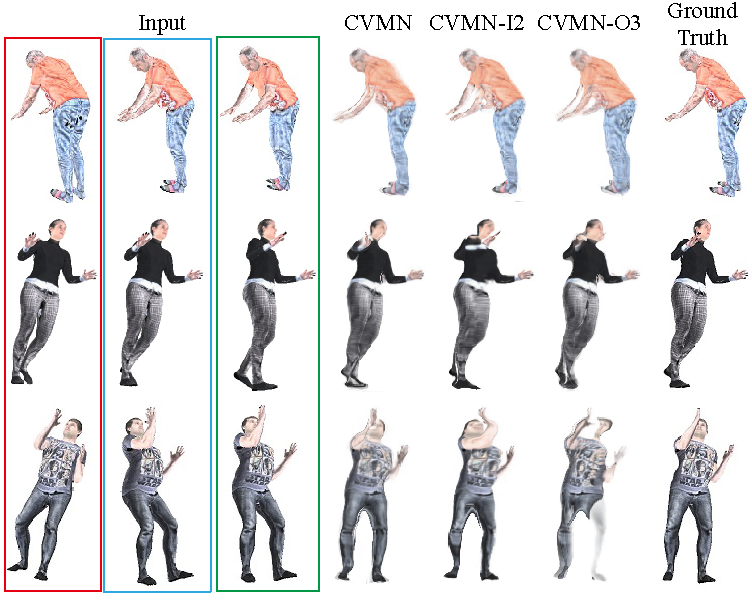
\includegraphics[width=\textwidth]{supplemental_surreal_I2_O3.pdf}
    \bicaption[CVMN与变体的对比结果图]{CVMN与变体的对比结果图。从左到右分别是:三个视角的输入参考图片,CVMN输出的结果,CVMN-I2输出的结果和CVMN-O3的输出结果。}{Qualitative comparison results for the ablation study. From left to right: the three input reference images, sample synthesized image by CVMN, CVMN-I2, and CVMN-O3, and the ground truth view.}
    \label{fig:cvmn_i2_o3}
\end{figure}
比较这些结果可以发现CVMN的瑕疵更少,与真实参考图片更接近。另外两个变体在发生遮挡变化的区域附近则出现了明显的瑕疵,直接说明了编码器提取特征过程中中间图像的巨大作用,以及解码过程中中间图像应该去掉,否则会将合成过程变得更加复杂而具有歧义。

\subsection{CVMN与DVM的比较}
DVM\citep{Ji_2017_CVPR}同样是利用深度学习求解视角插值的最新方法,由于原作者并未开源代码,实验中是按照原论文的描述复现了算法。考虑到DVM仅能插值两张图片正中间的视角,在SURREAL数据集上进行对比时,从$\mathcal{S}=\{\mathcal{C}_1, \mathcal{C}_2, \dots, \mathcal{C}_{24}\}$中随机选取一对图片$(\mathcal{C}_a, \mathcal{C}_b)$作为DVM的输入,同时选择$\mathcal{C}_{\lfloor (a+b)/2\rfloor}$作为监督数据。定量数据结果如表~\ref{tab:cvmn_surreal}最后一列所示,图~\ref{fig:cvmn_dvm}展示了出了部分插值出的新视角结果,本方法的效果明显优于DVM。从图中可以看出,DVM合成的图像重影和模糊现象比较严重,这是由于DVM无法应对大视角范围下的复杂遮挡变化问题,这在图中人物手臂的部分尤为明显。
\begin{figure}[!htbp]
    \centering
    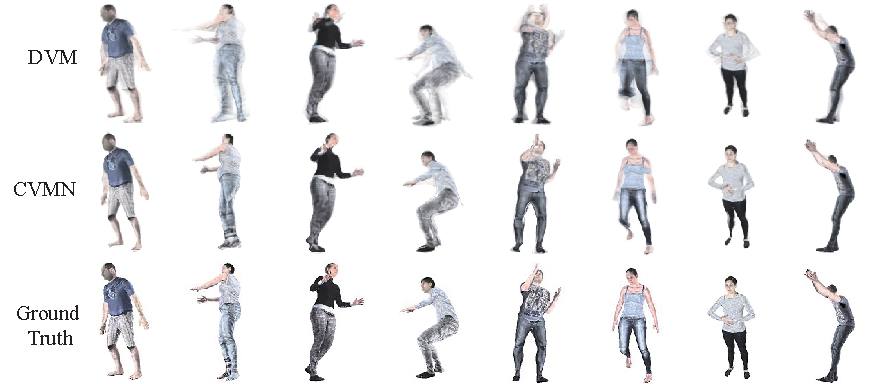
\includegraphics[width=\textwidth]{surreal_compare_DVM_1.pdf}
    \bicaption[与DVM比较的结果图]{与DVM比较的结果图。CVMN的输出图片中选取了中间的视角与DVM比较。}{Comparison with DVM. The middle view is picked in the synthesized sequence from CVMN to compare with DVM.}
    \label{fig:cvmn_dvm}
\end{figure}

\section{ShapeNet数据集实验}
为了进一步说明本方法的通用性,本节介绍在ShapeNet数据集\citep{shapenet2015}上的实验结果,以证明本方法对基本任意类型的3D对象都能表现很好。具体来说,本实验从整个ShapeNet数据集中挑选出汽车和椅子模型进行测试。数据的准备过程类似于之前对SURREAL所作的操作。视角变化的范围设定在30度到90度之间。用于测试的数据量为百分之二十,其余数据用于训练。用于训练的数据组数对于汽车模型和椅子模型分别是约10万组和20万组。训练过程与SURREAL设置一致。

在ShapeNet数据集上,本方法与包括DVM\citep{Ji_2017_CVPR},TVSN\citep{tvsn_cvpr2017}以及VSAF\citep{zhou2016view}在内的三个最新方法进行了定性和定量的比较实验。对于VSAF和TVSN,本实验采取了原作者提供的预训练模型。在渲染它们的测试数据时,插值视角范围从$\{40^\circ, 60^\circ, 80^\circ\}$中选取,使得测试角度在真实图片中有精确对应,从而保证比较的公平性。本实验使用MAE作为误差度量,实验数据结果如表~\ref{tab:cvmn_shapenet}所示。
\begin{table}
\bicaption[ShapeNet数据集上的定量指标数据]{ShapeNet数据集上的定量指标数据。}[Quantitative evaluation on the ShapeNet dataset]{Quantitative evaluation on the ShapeNet dataset.}
\label{tab:cvmn_shapenet}
\centering
\footnotesize% fontsize
\setlength{\tabcolsep}{4pt}% column separation
\renewcommand{\arraystretch}{0.9}%row space 
\begin{tabular}{c c c c c}
\hline\noalign{\smallskip}
Method  & DVM\citep{Ji_2017_CVPR} & VSAF\citep{zhou2016view} & TVSN\citep{tvsn_cvpr2017}& CVMN \\
\noalign{\smallskip}
\hline
\noalign{\smallskip}
Car   & 3.441 & 7.828 & 5.380 & \textbf{1.608}\\
Chair & 5.579 & 20.54 & 10.02 & \textbf{2.777}\\
\hline
\end{tabular}
\end{table}
部分可视化对比结果如图~\ref{fig:cvmn_shapenet}所示。TVSN在椅子数据上的结果表现比较差,而DVM仍然有明显的重影瑕疵。VSAF的可视化效果比其他方法差得较多,没有在图中展示。本方法在椅子和汽车类别下均能较好地合成新视角,生成的插值图像能够较好地接近真实数据。
\begin{figure}[!htbp]
    \centering
    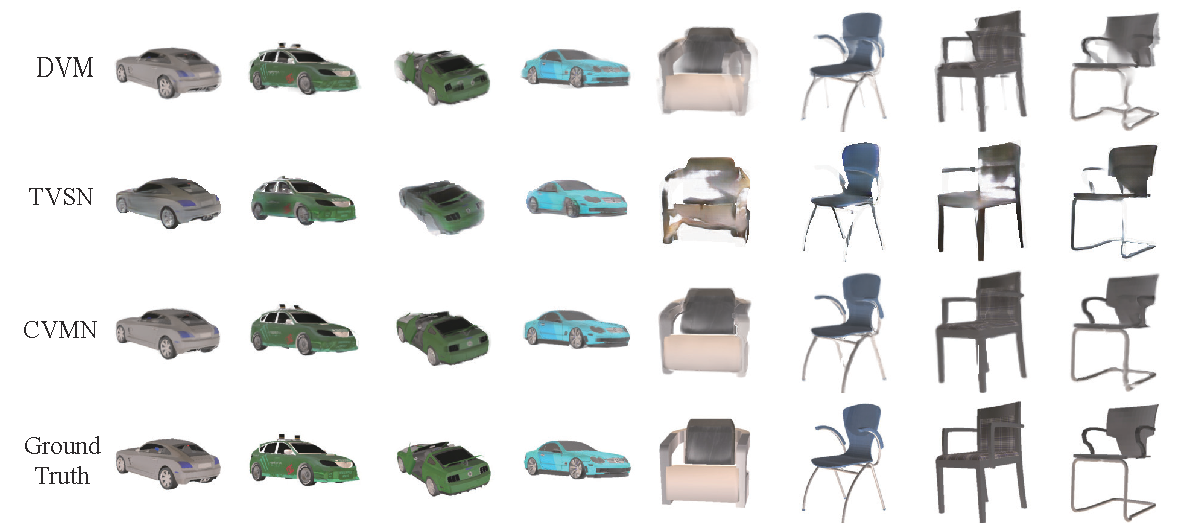
\includegraphics[width=\textwidth]{shapenet_result_1.pdf}
    \bicaption[ShapeNet数据集上的可视化结果对比图]{ShapeNet数据集上的可视化结果对比图。}{Quanlitative comparisons with DVM and TVSN on ShapeNet.}
    \label{fig:cvmn_shapenet}
\end{figure}

\section{真实场景实验}
本节介绍真实场景下的动作序列实验。用来采集真实数据的采集系统是一个专门搭建的三摄像机系统。所使用的工业相机使用网线连接到一台采集服务器,同时使用硬件触发进行同步。相机围绕拍摄对象距离约3米左右,三个相机使用多视角视图配准(SfM)进行标定。为了测试不同视角范围下的输入,捕捉不同序列的时候相机的位置进行了移动。总的来说,左右摄像机之间的视角变换在30度到60度之间。

对采集得到的图像,首先进行预处理,利用预先标定的内参去除相机畸变,并使用背景减除算法移除背景。然后利用环形校正或者对齐到圆环上的三元组。最终,将弧三元组喂给CVMN网络来合成新的视角序列。由于缺乏真实标注数据用于监督训练,本实验中的网络参数使用的是在SURREAL数据集\cite{varol2017}上训练的结果。图~\ref{fig:cvmn_real}展示了合成结果。尽管真实数据由于噪声、高动态范围和光照的剧烈变化而更具挑战性,但是在仿真数据集上训练出的网络参数依然可以产生高质量的合成插值结果。这表面本方法的准确性和健壮性都很好。图中也与DVM的结果进行了对比,其重影瑕疵由于大视角的变化,依然很明显。
\begin{figure}[!htbp]
    \centering
    \includegraphics[width=\textwidth]{real_scene_qualitative-eps-converted-to.pdf}
    \bicaption[ShapeNet数据集上的可视化结果对比图]{真实数据结果图。挑出了合成序列中的四张展示出来。DVM合成的中间视角显示在最右边一列。}{Real scene results. Four samples from the morphing sequence. The middle view synthesized by DVM is shown on the right column.}
    \label{fig:cvmn_real}
\end{figure}

\section{子弹时间效果的渲染结果}
本节介绍利用提出的环形视角变换方法实现“子弹时间”效果的实验。由于合成的图片序列是已经对齐到一个理想圆环上的,所以本身非常适合通过多次变换相邻的视图三元组,来创建子弹时间。本实验仍然在SURREAL数据集上完成,从围绕一个对象拍摄一圈的相机角度中选出6组环上的图片三元组,实验中规定相邻的两组三元组会共享一张图,总计就是12张图。对每一组环上的三元组,利用本方法生成变换序列,然后连接在一起,就构成了完整的一整圈视角。图~\ref{fig:bullet_time}展示了部分实例图像。
\begin{figure}[!htbp]
    \centering
    \includegraphics[width=\textwidth]{bullet_time-eps-converted-to.pdf}
    \bicaption[子弹时间效果渲染图]{子弹时间效果渲染图。图中展示了144个渲染视角中的21个,图的右边显示Visual hull 得到的几何模型效果。}{Bullet-time effect rendering result. Showing 21 samples out of the the 144 views in the bullet-time rendering sequence. Visual hull reconstruction from the view sequence is shown on the right.}
    \label{fig:bullet_time}
\end{figure}

图的右边同时展示了用全部的插值图像的轮廓信息计算出的人的三维模型。观察模型可以发现,人的大致几何是能够恢复出来,但是包括面部、手脚和身上衣服的纹理细节是缺失的。在本文算法的章节中提到了CVMN中用来表示隐式几何的运动偏移向量场和可见性蒙版,这里恢复出的几何正好印证了渲染图片质量与隐式几何表达之间的联系。在渲染任务中,关注的重点在于渲染结果而不是几何,本实验部分地论证了渲染结果的提升不一定要完全依赖精确的几何,即粗略的几何模型很可能已经满足渲染需求,但同时几何表达对于图片信息的融合也不可或缺,毕竟在本实验中仅仅对图片进行监督实际上足以得到大致准确的几何模型。

\section{本章小结}
本章介绍了环形视角变换方法在多个数据集上的实验结果。通过在仿真的人体和一般物体的数据上测试,说明了提出的方法具有普适性。通过在真实数据上的测试,说明了提出的方法具有泛化性和鲁棒性,尤其是CVMN网络模块的设计遵循奥卡姆剃刀原则。在与其他的视角变换及合成算法的对比中,效果超越了其他方法。最后展示了“子弹时间”效果以及利用合成的新图片反过来重建出了几何模型,说明了隐式几何表达在本方法中的必要性,同时讨论了几何先验在渲染任务中既不可或缺又可一定程度上折衷的辩证思想。

